\documentclass[10pt]{article}

% ---- NeurIPS-preprint-style layout ----------------------------------------
\usepackage[letterpaper,textwidth=5.5in,textheight=9in,centering]{geometry}
\usepackage{times}
\usepackage[T1]{fontenc}
\usepackage[utf8]{inputenc}
\usepackage{microtype}
\usepackage{graphicx}
\usepackage{booktabs}
\usepackage{amsmath}
\usepackage{xcolor}
\usepackage{caption}
\usepackage{tikz}
\usetikzlibrary{arrows.meta,positioning,fit}
\usepackage[colorlinks=true,linkcolor=black,citecolor=black,urlcolor={rgb,255:red,146;green,64;blue,14}]{hyperref}

\captionsetup{font=small,labelfont=bf,skip=6pt}
\newcommand{\head}[1]{\textbf{#1}}
\definecolor{amber}{RGB}{201,123,34}
\definecolor{boxbg}{RGB}{252,247,238}

\usepackage{titlesec}
\titlespacing*{\section}{0pt}{14pt}{6pt}
\titlespacing*{\subsection}{0pt}{10pt}{4pt}
\titleformat*{\section}{\large\bfseries}
\titleformat*{\subsection}{\normalsize\bfseries}

\usepackage{abstract}
\renewcommand{\abstractnamefont}{\normalfont\bfseries}
\renewcommand{\abstracttextfont}{\normalfont\small}

\title{\bfseries MLPal Gateway: Curation Over Breadth\\in a Self-Hostable AI Gateway}
\author{Sai Vivek Peddi\\MLPal \and Claude\\\textit{benchmark harness \& analysis}}
\date{Technical report v2 --- August 12, 2026\\[2pt]\small Measurements executed 11--12 August 2026 unless dated otherwise.\\\small Code, harness, and raw results: \href{https://github.com/ML-Pal/mlpal-gateway}{\texttt{github.com/ML-Pal/mlpal-gateway}} (Apache-2.0)}

\begin{document}
\maketitle

\begin{abstract}
AI gateways compete on catalog breadth: OpenRouter advertises 400+ models, Portkey 1{,}600+, LiteLLM 100+ providers [1,7,5]. We argue breadth is the wrong metric. Production models now retire on a $\sim$12-month cycle --- Gemini~1.5 snapshots lived exactly 12 months, Claude Opus~4.1 was retired one year to the day after release, GPT-4.5-preview survived 4.5 months, and AWS Bedrock has made a 12-month platform lifetime \emph{contractual} [9,11,12,14] --- so a large catalog is mostly retired-or-dominated inventory, while gateway utility concentrates in whether current models are served well and references to them survive churn. We present \textbf{MLPal Gateway}, an open-source (Apache-2.0), self-hostable gateway built on this hypothesis: a curated catalog (73 models served in production) behind an Anthropic-wire core, \emph{availability-aware router tags} that resolve a stable alias to the best model a deployment can actually serve, pass-through compute-unit metering, and per-key policy, budgets, and cache/latency observability. We measure it four ways. \textbf{(i)~Gateway overhead}, isolated against a zero-latency fake upstream ($N{=}100$ per system): \textbf{8.5\,ms} median added TTFT with the full admission pipeline enabled --- faster than a LiteLLM proxy in both its bare configuration (13.2\,ms) and a matched production configuration with database-backed virtual keys, budgets, and spend tracking (15.3\,ms), with the tightest tail (p95 33 vs.\ 58/41\,ms). We document the three engineering changes that took our overhead from 20.3\,ms to 8.5\,ms. \textbf{(ii)~Client-observed latency}: a CloudFront edge cutover executed during this study reduced production median TTFT from 871\,ms to \textbf{642\,ms}; a same-night four-way benchmark places OpenRouter at 898\,ms on the identical model and vantage. \textbf{(iii)~Provider-semantics preservation}: prompt caching passes through byte-faithfully (22k-token prefix, write$\rightarrow$read on all systems) and metered cost reproduces the provider's list price to five decimals, falling 12.3$\times$ on cache hits. \textbf{(iv)~System-level utility}: a coding agent routing sub-tasks via the gateway catalog cut sub-agent cost $\sim$10$\times$ at near-matched correctness. We release the gateway, console, SDK, and the full reproduction harness.
\end{abstract}

\section{Introduction}
An AI gateway multiplexes model providers behind one API and one billing relationship. The category has consolidated around a breadth race: OpenRouter's pricing page advertises 400+ models across 70+ providers [1]; Portkey's gateway README claims routing to 1{,}600+ models [7]; LiteLLM supports 100+ providers [5]. Model count is legible and easy to market --- and, we argue, largely disconnected from delivered utility.

Our hypothesis is that \textbf{provider agnosticism matters, but breadth does not}: models are retiring at a record and accelerating pace (\S\ref{sec:curation}), so most of a large catalog is dead or dominated weight, while real traffic concentrates on a small set of current models per provider. What a practitioner needs from a gateway is (a)~that current models are served correctly --- valid parameter ranges, caching, streaming fidelity, provider quirks handled per model; (b)~that their own code survives retirements without edits; and (c)~that the cost and behavior of every request is observable. Each is a per-model investment that scales to tens of models, not thousands.

This report contributes:
\begin{enumerate}\itemsep2pt
\item A quantified case that model lifetimes have compressed toward $\sim$12 months, from providers' own deprecation ledgers (\S\ref{sec:curation}, Fig.~\ref{fig:lifetimes}).
\item The system design: an Anthropic-wire universal core with OpenAI-compatible endpoints, availability-aware router tags, pass-through compute-unit metering, and per-key admission --- one codebase serving both a managed deployment and a self-hosted open-source distribution (\S\ref{sec:design}).
\item Controlled measurements with a fair baseline: gateway overhead isolated against a zero-latency upstream, compared to LiteLLM in \emph{both} bare and matched production configurations (\S\ref{sec:overhead}); a client-observed latency decomposition and the measured effect of an edge cutover executed mid-study (\S\ref{sec:client}); a same-night four-way comparison including OpenRouter (\S\ref{sec:openrouter}); cache and metering fidelity verified from the wire (\S\ref{sec:fidelity}); and system-level routing utility on a coding-agent workload (\S\ref{sec:utility}).
\item The performance-engineering record: the three changes that halved our hot-path overhead, each verified by trace inspection (\S\ref{sec:engineering}).
\end{enumerate}

\section{The case for curation}\label{sec:curation}
\head{Model lifetimes are compressing.} Fig.~\ref{fig:lifetimes} plots launch-to-retirement spans for twelve production API models from providers' own lifecycle pages [9,11,12,13,14]. The 2024 cohort lived 22--29 months; the 2025 cohort converges on 12--16; GPT-4.5-preview --- flagship-priced --- survived \textbf{4.5 months} with a 91-day removal notice [9]. Google's numbered Gemini snapshots retired exactly 12 months after release (1.5-pro-001: 2024-05-24$\rightarrow$2025-05-24; -002: 2024-09-24$\rightarrow$2025-09-24) [12]. Claude Opus~4.1 was retired one year to the day after release (2025-08-05$\rightarrow$2026-08-05) with a $\sim$61-day notice [11,16]. Notice windows compressed in parallel: Anthropic's 2025 retirements carried $\sim$181-day notices, its 2026 cohort $\sim$61 days [11,16]; OpenAI's policy floor is six months for GA models and \emph{three} for specialized variants [9].

\begin{figure}[t]
\centering
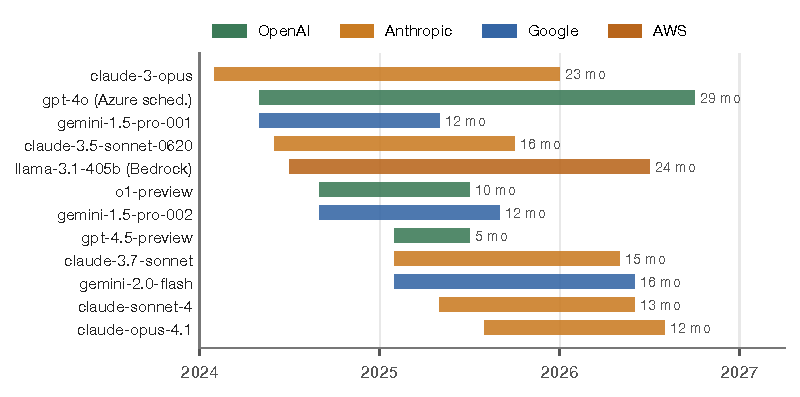
\includegraphics[width=\linewidth]{fig-lifetimes.pdf}
\caption{Launch$\rightarrow$retirement spans for production API models, ordered by launch date, from official provider lifecycle pages [9,11,12,13,14] (gpt-4o shows Microsoft's published Azure retirement schedule; Bedrock dates are platform-specific). Models launched in 2024 lived 22--29 months; models launched in 2025 live 12--16.}
\label{fig:lifetimes}
\end{figure}

\head{Churn is now contractual.} AWS Bedrock's lifecycle policy guarantees only 12 months of platform availability after launch, moves models to a Legacy state in which an account inactive on that model for 15 days loses access, and (for post-2026 EOLs) adds an extended-access phase at \emph{provider-set higher pricing} [14]. Deprecation is a scheduled property of the substrate, not an exceptional event.

\head{Retirement breaks production.} When OpenAI removed GPT-4o from ChatGPT at GPT-5's launch with zero notice (2025-08-07), user revolt forced reinstatement within five days [10,15]; the February-2026 retirement wave left some business customers without model access for a week [10]. On Claude Opus~4.1's retirement day, hard-coded model IDs failed simultaneously across Bedrock, Vertex, and the first-party API, and migration was complicated by a breaking parameter change in the successor [16].

\head{Serving a model well is per-model work.} Extracting a model's best behavior requires model-specific handling a lowest-common-denominator passthrough cannot provide: reasoning-budget ranges that are discontinuous and differ per model (we maintain per-model valid ranges for Gemini's \texttt{thinking\_budget}); prompt-cache minimums that differ per model (a $\sim$2.5k-token prefix silently fails to cache on claude-haiku-4.5, whose minimum is 4{,}096 tokens --- the request succeeds and bills full price); parameter support that changes across successors [16]; and per-provider streaming and error quirks. This scales to a curated set. The right unit of comparison is \emph{utility per supported model}, not the count.

\section{System design}\label{sec:design}

\begin{figure}[t]
\centering
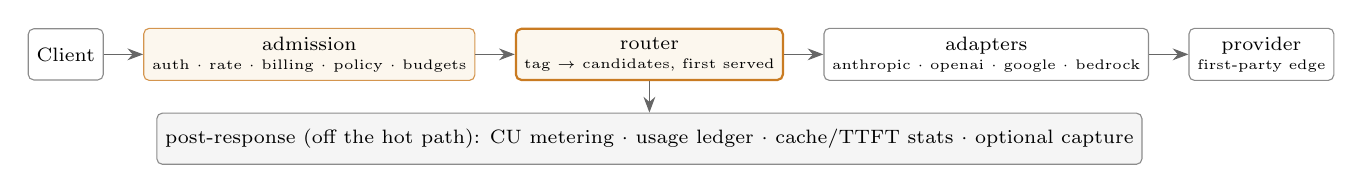
\begin{tikzpicture}[
  font=\scriptsize,
  box/.style={draw=black!45, rounded corners=2pt, minimum height=6.5mm, inner sep=3pt, fill=white},
  stage/.style={box, fill=boxbg, draw=amber!80},
  arr/.style={-{Stealth[length=2mm]}, black!60},
  lbl/.style={font=\tiny, text=black!55}
]
\node[box] (client) {Client};
\node[stage, right=5mm of client, align=center] (adm) {admission\\[-1pt]{\tiny auth $\cdot$ rate $\cdot$ billing $\cdot$ policy $\cdot$ budgets}};
\node[stage, right=5mm of adm, align=center, draw=amber, thick] (router) {router\\[-1pt]{\tiny tag $\to$ candidates, first served}};
\node[box, right=5mm of router, align=center] (adapters) {adapters\\[-1pt]{\tiny anthropic $\cdot$ openai $\cdot$ google $\cdot$ bedrock}};
\node[box, right=5mm of adapters, align=center] (prov) {provider\\[-1pt]{\tiny first-party edge}};
\node[box, below=4mm of router, align=center, fill=black!4] (post) {post-response (off the hot path): CU metering $\cdot$ usage ledger $\cdot$ cache/TTFT stats $\cdot$ optional capture};
\draw[arr] (client) -- (adm);
\draw[arr] (adm) -- (router);
\draw[arr] (router) -- (adapters);
\draw[arr] (adapters) -- (prov);
\draw[arr] (router) -- (post);
\end{tikzpicture}
\caption{Request path. Admission runs before routing; adapters translate to each provider's native API behind circuit breakers and relay SSE without re-chunking; metering, the usage ledger, and optional payload capture run after the response.}
\label{fig:arch}
\end{figure}

\subsection{One codebase, two deployments}
The managed service (\texttt{models.mlpal.ai}) and the open-source distribution (\texttt{mlpal-gateway}) are the same codebase. Deployment differences are confined to composition-root \emph{seams} --- auth backend, billing backend, payload-capture default (on for self-hosters operating their own box; off in the managed service, which retains billing metrics and never stores payloads) --- never forks. The distribution boots with one \texttt{docker compose up}; a catalog reconcile seeds the model registry, pricing, and routing feed; 341 unit tests and a console build gate CI.

\subsection{Wire surface}
The core endpoint is Anthropic-wire \texttt{POST /v1/messages} --- request/response envelopes, SSE event grammar, tool use, and \texttt{cache\_control} are Anthropic's, for every provider behind the gateway. OpenAI-compatible endpoints (\texttt{/v1/chat/completions}, embeddings, images, audio) serve existing OpenAI-SDK code unchanged. Every response carries its metered cost in an \texttt{X-MLPal-Compute-Units} header and a routing envelope naming the resolved model.

\subsection{Availability-aware router tags}
A router tag (\texttt{mlpal}, \texttt{mlpal-flash}, \texttt{mlpal-lite}) maps to a priority-ordered, provider-spanning candidate list maintained in the catalog feed. Resolution walks the list and picks the first candidate the \emph{local deployment} can serve (model active, not paused, provider key configured); the resolution is cached per instance and warmed at startup. A client that ships \texttt{"model": "mlpal"} survives every retirement in Fig.~\ref{fig:lifetimes} without a code change, and the mechanism degrades gracefully to single-provider deployments: a box with only an Anthropic key still resolves every tag. The same curated intelligence is exposed declaratively as a ranked catalog (\texttt{GET /v1/catalog}) for clients that choose their own model per task; \S\ref{sec:utility} measures that consumption mode.

\subsection{Metering: pass-through compute units}
Cost is metered in compute units pegged at 1~CU $=$ \$10 of provider list price:
$\mathrm{CU} = \sum_{c} \mathrm{tokens}_c \cdot \mathrm{rate}_c \,/\, 10$
over billing components $c$ (input; output; cache-write at the provider's 1.25$\times$ input rate; cache-read at 0.1$\times$). There is no markup term: self-hosters pay providers directly, and the managed tier bills tokens at cost with a flat platform fee, so the meter is an instrument, not a margin. The ledger stores CU at \texttt{numeric(24,12)}; \S\ref{sec:fidelity} verifies the meter against the wire. Per-key spend budgets (multiple sliding windows, checked at admission, never cutting a running stream) and model-policy globs complete the admission pipeline; per-key aggregates expose cache hit rate, latency p50/p95, time-to-first-token, and stream share.

\section{Experimental setup}\label{sec:setup}
\head{Overhead study (\S\ref{sec:overhead}).} To isolate gateway overhead from provider variance, all gateways are pointed at a \emph{fake upstream}: a local HTTP server answering \texttt{/v1/messages} with a canned, valid Anthropic streaming response (14 SSE events, 9 content deltas) with zero think time. Four systems, $N{=}100$ streaming trials each, order-rotated: (a)~the fake upstream called directly (client+server floor); (b)~\textbf{MLPal Gateway} (Docker, full admission: key auth, Redis rate limiting, billing gate, model policy, budget windows, metering, usage persistence, payload capture on); (c)~\textbf{LiteLLM bare} (\texttt{ghcr.io/berriai/litellm:main-latest}, pulled 2026-08-11; static master-key auth, no database); (d)~\textbf{LiteLLM production config}: the same image with PostgreSQL-backed virtual keys --- the benchmark authenticates with a generated virtual key carrying a model allowlist, budget, and rpm limit, with spend tracking enabled. Configuration (d) is the fair comparison: it is LiteLLM doing the same class of per-request work as (b).

\head{Client-observed study (\S\ref{sec:client}--\ref{sec:openrouter}).} Same protocol as our July study [17]: identical prompt ($\sim$150-word CAP-theorem task), \texttt{max\_tokens} 256, streaming, one cold connection per request, one unmeasured warmup, $N{=}15$ per system, A/B rotation, 0.5\,s spacing, model snapshot \texttt{claude-haiku-4-5-\allowbreak 20251001} everywhere (OpenRouter: \texttt{anthropic/claude-haiku-4.5}, OpenAI wire). Metrics: TTFB (first SSE byte), TTFT (first content token), total, content-chunk count. Client: Apple-silicon macOS, Python httpx, residential network. Server-side ground truth comes from AWS X-Ray traces of the production service.

\head{Cache experiment (\S\ref{sec:fidelity}).} A $\sim$22k-token system prefix marked \texttt{cache\_control: ephemeral} (above haiku-4.5's 4{,}096-token minimum), distinct per system so systems cannot share provider cache entries; four sequential non-streaming trials per system against the real provider; usage fields read from the wire; metering fidelity verified by reading the CU header on a cache-write and cache-read call of the same prefix.

\section{Results}
Table~\ref{tab:matchups} orients the section: each comparison is like-for-like --- our open-source gateway against the open-source proxy a self-hoster would otherwise deploy, and our managed service against the managed gateway a team would otherwise buy --- plus the raw-provider floor that bounds what any gateway can achieve.

\begin{table}[t]
\centering\small
\caption{The comparisons in this report, like-for-like. Each row names the deployment class, the contender, and the headline result; details in the referenced sections.}
\label{tab:matchups}
\setlength{\tabcolsep}{4pt}
\begin{tabular}{p{2.9cm}p{3.3cm}p{6.4cm}}
\toprule
Matchup & Systems & Headline result \\
\midrule
Self-hosted vs.\ self-hosted (\S\ref{sec:overhead}) & MLPal Gateway (OSS) vs.\ LiteLLM proxy (OSS), bare and production configs & MLPal +8.5\,ms overhead with full admission vs.\ +13.2 (bare) / +15.3 (production); p95 33 vs.\ 58 / 41\,ms ($N{=}100$) \\[2pt]
Managed vs.\ managed (\S\ref{sec:openrouter}) & \texttt{models.mlpal.ai} vs.\ OpenRouter, same model/night/vantage & MLPal 642\,ms median TTFT vs.\ 898; p95 957 vs.\ 1{,}424 ($N{=}15$); OpenRouter streams finer chunks (93 vs.\ 9) \\[2pt]
Managed vs.\ raw provider (\S\ref{sec:client},\S\ref{sec:openrouter}) & \texttt{models.mlpal.ai} vs.\ direct \texttt{api.anthropic.com} & +99\,ms at the median (642 vs.\ 543) buys routing, metering, policy, and observability \\[2pt]
Semantics fidelity (\S\ref{sec:fidelity}) & MLPal, LiteLLM, direct & prompt caching byte-faithful on all three; MLPal's meter reproduces list price to five decimals \\[2pt]
Broader managed study [17] & MLPal vs.\ OpenRouter, 11 model pairs (July 2026) & MLPal won median TTFT 8/11 with tighter tails; OpenRouter won throughput and fast/cheap models; neither dominated \\
\bottomrule
\end{tabular}
\end{table}

\subsection{Self-hosted head-to-head: MLPal Gateway vs.\ LiteLLM (gateway overhead)}\label{sec:overhead}

\begin{figure}[t]
\centering
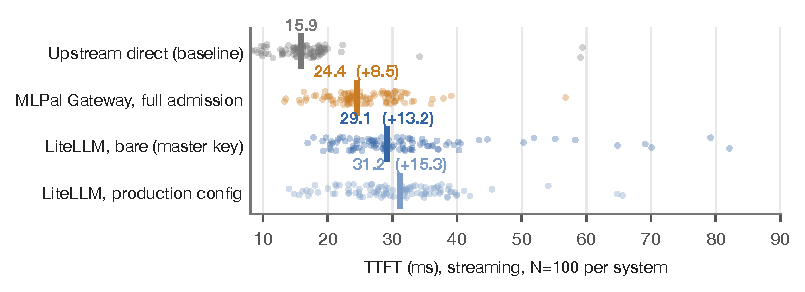
\includegraphics[width=\linewidth]{fig-synth.pdf}
\caption{Added latency isolated: per-trial TTFT against a zero-latency fake upstream ($N{=}100$ per system, streaming; bar $=$ median, label $=$ median (delta vs.\ baseline)). MLPal Gateway with its full admission pipeline undercuts LiteLLM in both its bare (master-key) and production (database-backed virtual keys, budgets, spend tracking) configurations.}
\label{fig:synth}
\end{figure}

\begin{table}[t]
\centering\small
\caption{Overhead study, $N{=}100$ streaming trials per system against the fake upstream (medians; $\Delta$ vs.\ the direct-call baseline). All three gateways preserve the 9-chunk stream exactly.}
\label{tab:synth}
\begin{tabular}{lrrrr}
\toprule
System & TTFT med (ms) & $\Delta$ med & p95 & total med \\
\midrule
Upstream direct (baseline) & 15.9 & --- & 20.0 & 16.2 \\
\textbf{MLPal Gateway, full admission} & \textbf{24.4} & \textbf{+8.5} & \textbf{33.3} & 30.4 \\
LiteLLM, bare (master key) & 29.1 & +13.2 & 58.3 & 29.4 \\
LiteLLM, production config & 31.2 & +15.3 & 41.1 & 31.5 \\
\bottomrule
\end{tabular}
\end{table}

Table~\ref{tab:synth} and Fig.~\ref{fig:synth} give the central result: with authentication, rate limiting, billing gate, model policy, budget windows, metering, and payload capture all enabled, MLPal Gateway adds \textbf{8.5\,ms} at the median --- less than LiteLLM checks a single static string for (13.2\,ms), and 6.8\,ms less than LiteLLM doing comparable per-request work (15.3\,ms). The tail is more decisive: p95 of 33\,ms vs.\ 58\,ms (bare) and 41\,ms (production). Against a real $\sim$3\,s completion, all of these are noise; the result matters because it removes the standing excuse that governance costs latency --- admission-time policy, budgets, and metering are computationally free at gateway scale.

\subsection{How the overhead was halved}\label{sec:engineering}
Our first measurement of this experiment gave \textbf{20.3\,ms} --- \emph{slower} than bare LiteLLM (13.4\,ms). Three changes, each identified from AWS X-Ray traces of the production service and re-verified after deployment, took it to 8.5\,ms:
\begin{enumerate}\itemsep2pt
\item \head{Connection pooling to the provider.} The Anthropic edge constructed a new HTTP client --- and therefore a fresh TCP+TLS handshake to the provider --- on \emph{every request}. Replaced with a per-event-loop pooled client. This is the largest single saving and also removes a per-request handshake from the production path to \texttt{api.anthropic.com}.
\item \head{Pure-ASGI observability.} Two Starlette \texttt{BaseHTTPMiddleware} layers each wrapped every response in an extra task and memory stream (a scheduling hop on every streamed chunk, including the first token), and one parsed the \emph{entire} request body with \texttt{json.loads} solely to read the model name for a metrics label --- a double full-body parse on multi-hundred-kilobyte agentic payloads. Replaced by a single pure-ASGI middleware that never buffers or re-parses the body (the model dimension comes from a bytes-regex on the first chunk) and emits metrics only after the response has started.
\item \head{Timer-free relay.} The SSE relay awaited \texttt{wait\_for(queue.get(), timeout)} per chunk --- a timer plus exception-based control flow on every event --- to inject keepalive pings during provider silence. Replaced by a single idle-ping task; chunks now cross one queue hop with no timer.
\end{enumerate}
Post-deployment X-Ray traces confirm the structure: all admission I/O completes by $+8.6$\,ms (the previously serialized Redis calls now visibly overlap; budget windows are read in one pipelined round trip), the provider call fires at $+19.5$\,ms, and metering/accrual appear only after the response. An isolated probe of the admission pipeline (full stack, no provider call) measures \textbf{2.7\,ms} median on the local box and $\sim$12\,ms warm on production (in-VPC Redis/database hops).

\subsection{Client-observed latency and the edge cutover}\label{sec:client}

\begin{table}[t]
\centering\small
\caption{Network-layer cost to each host from the client vantage (median of 5 cold probes, 2026-08-11), before and after the CloudFront cutover executed during this study.}
\label{tab:network}
\begin{tabular}{lrrr}
\toprule
Host & TCP (ms) & TLS done (ms) & \texttt{/health} TTFB (ms) \\
\midrule
\texttt{models.mlpal.ai} (direct ALB, before) & 75 & 250 & 380 \\
\texttt{models.mlpal.ai} (CloudFront, after) & \textbf{11} & \textbf{32} & \textbf{94} \\
\texttt{api.anthropic.com} (reference) & 12 & 26 & 40 \\
\bottomrule
\end{tabular}
\end{table}

From this vantage, the managed service's latency gap over direct provider access was dominated by geography, not software: a single-region ALB cost $\sim$75\,ms TCP and $\sim$250\,ms TLS per cold connection, against a CDN edge $\sim$12/26\,ms away (Table~\ref{tab:network}); the service itself contributes $\sim$20\,ms (\S\ref{sec:engineering}). Our July report [17] predicted that edge termination would recover this tax; during this study we executed the cutover --- \texttt{models.mlpal.ai} now resolves to CloudFront in front of the same ALB, with streaming validated end-to-end before the DNS change (the gateway's 15\,s SSE heartbeat keeps long streams under CloudFront's 60\,s origin idle timeout). Measured effect on the full request path ($N{=}15$, same night): median TTFT \textbf{871\,ms $\rightarrow$ 642\,ms}, p95 1{,}357--2{,}613 $\rightarrow$ 957\,ms. Existing clients required no changes.

\subsection{Managed head-to-head: MLPal vs.\ OpenRouter, same night}\label{sec:openrouter}

\begin{figure}[t]
\centering
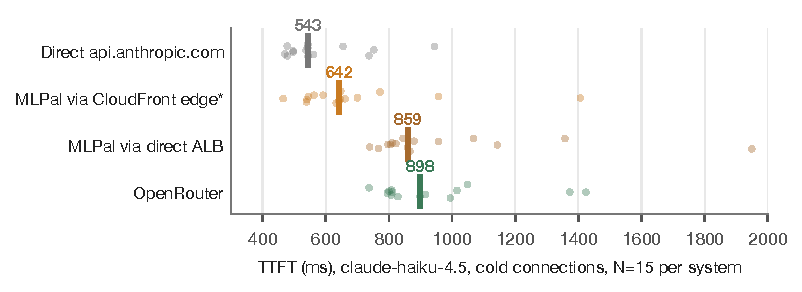
\includegraphics[width=\linewidth]{fig-vantage.pdf}
\caption{Client-observed TTFT on \texttt{claude-haiku-4.5}, cold connections, $N{=}15$ per system, all runs within the same evening from the same client. *The CloudFront row was measured $\sim$40 minutes after the other three (post-cutover); Anthropic-side variance was elevated all evening, so cross-row deltas carry $\sim\pm$50\,ms of session noise.}
\label{fig:vantage}
\end{figure}

\begin{table}[t]
\centering\small
\caption{Same-night comparison ($N{=}15$ each, streaming, cold connections, identical prompt and model snapshot). OpenRouter serves $\sim$93 fine-grained chunks vs.\ Anthropic's $\sim$9 coarse chunks through both MLPal paths --- the chunking difference of [17] persists.}
\label{tab:fourway}
\begin{tabular}{lrrrr}
\toprule
Path & TTFT med (ms) & p95 & total med & chunks med \\
\midrule
Direct \texttt{api.anthropic.com} & 543 & 944 & 3{,}051 & 9 \\
\textbf{MLPal via CloudFront edge} & \textbf{642} & \textbf{957} & 3{,}134 & 9 \\
MLPal via direct ALB (pre-cutover) & 859 & 1{,}357 & 3{,}459 & 10 \\
OpenRouter & 898 & 1{,}424 & 3{,}155 & 93 \\
\bottomrule
\end{tabular}
\end{table}

With an OpenRouter key supplied for this study we re-ran the head-to-head on the same model, vantage, and evening (Table~\ref{tab:fourway}). Post-cutover, the managed service leads OpenRouter by $\sim$250\,ms at the median and $\sim$470\,ms at p95 on this model, and sits $\sim$100\,ms behind direct provider access --- the residual being client$\to$edge$\to$us-east-2$\to$provider geography plus $\sim$20\,ms of service time. OpenRouter retains the finer-grained stream (93 vs.\ 9 chunks; upstream Anthropic chunks coarsely on our route, a perceived-smoothness advantage for OpenRouter in interactive UIs). Our July study [17], with its eleven model pairs, remains the broader comparison: OpenRouter won median TTFT on fast/cheap models near its edge and sustained higher steady-stream throughput, while MLPal won every Anthropic pair with substantially tighter tails; neither system dominated. Those results predate both this study's engineering and OpenRouter's own evolution since July.

\subsection{Provider semantics survive the hop: caching and metering fidelity}\label{sec:fidelity}

\begin{figure}[t]
\centering
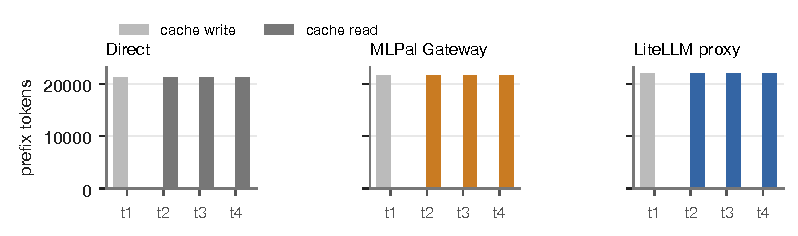
\includegraphics[width=\linewidth]{fig-cache.pdf}
\caption{Prompt-cache passthrough: $\sim$22k-token prefix with \texttt{cache\_control}, four sequential trials per system, distinct prefixes per system. Every system shows the canonical pattern --- full write on trial~1, full read on trials~2--4.}
\label{fig:cache}
\end{figure}

Prompt caching is the highest-leverage provider feature a gateway can break silently: reordering or rewriting the prefix destroys cache identity and the client pays full price with no error. All three systems preserved it exactly (write of 21{,}213--22{,}013 tokens on trial~1; reads of the identical count after; Fig.~\ref{fig:cache}). On MLPal, the meter tracked it end-to-end: the cache-write call metered \textbf{0.002756~CU} and the cache-read call \textbf{0.000224~CU} --- a \textbf{12.3$\times$} reduction, each figure reproducing Anthropic's list price exactly ($22{,}013 \times 1.25 \times \$1/\mathrm{M} \div \$10 = 0.00275$; $\times\,0.1$ for reads $= 0.00022$) [19]. The meter is verified from the wire, not from our own configuration. Cache read/write tokens land in each usage row; per-key cache hit rate is a first-class dashboard metric (an agentic coding workload on our development deployment sustains 44\%).

\subsection{Utility over breadth at the system level}\label{sec:utility}
The curation thesis predicts that a ranked, current catalog beats a large flat one for real workloads. A measurement from our coding agent (yodex, 2026-07-28 [18]): on a four-module build with delegation, the agent consulted the gateway catalog to route each sub-task by rated complexity --- trivial modules to \texttt{gemini-2.5-flash-lite}, harder ones upward --- cutting sub-agent cost \textbf{$\sim$10$\times$} (0.212$\rightarrow$0.022~CU) versus inheriting the pinned frontier model, at near-matched correctness (11/12 vs.\ 12/12), and $\sim$2$\times$ cheaper end-to-end than a same-model Claude Code baseline. The enabling primitive is a catalog small enough to rank honestly and current enough to trust.

\section{Feature comparison}\label{sec:features}

\begin{table}[t]
\centering\scriptsize
\caption{Feature surfaces from current public documentation (retrieved 2026-08-11) [1,2,4,5,6,7,8] and MLPal source [3]. ``---'' $=$ not offered/documented; \emph{italics} $=$ the vendor's hosted/enterprise tier rather than the OSS artifact. LiteLLM's OSS proxy \emph{does} provide key management, budgets, and callback-based logging (\S\ref{sec:setup}, config d); the differences below are of integration and defaults, not existence.}
\label{tab:features}
\setlength{\tabcolsep}{3.5pt}
\begin{tabular}{p{2.35cm}p{2.5cm}p{2.3cm}p{2.15cm}p{2.05cm}p{2.6cm}}
\toprule
Dimension & OpenRouter & LiteLLM (OSS) & Portkey (OSS) & Helicone & MLPal Gateway \\
\midrule
Catalog & 400+ models, 70+ providers & 100+ providers & 1{,}600+ models claimed & 100+ models & 55 curated entries; 73 served (managed) \\
Self-host & --- & MIT & MIT & Apache-2.0 (cloud-primary) & Apache-2.0 core \\
Anthropic-wire endpoint & --- (OpenAI wire + Responses beta) & yes & not documented & not documented & core surface, all providers \\
Fee model & 5.5\% on credits & free / quote enterprise & free / \$49+ hosted logs & 0\% + Stripe & free self-host; managed: tokens at cost + flat fee \\
Stable model alias & auto-router & operator-defined config & configs/routing rules & --- & curated, availability-aware, feed-updated \\
Multi-provider fallback & yes, price-weighted & yes (strategies) & yes & yes & --- (one pinned first-party edge per model) \\
Per-request cost on wire & via /generation lookup & cost tracking (DB) & \emph{hosted} & registry-computed & CU header, every response, meter-verified (\S\ref{sec:fidelity}) \\
Per-key cache/TTFT/tail metrics & activity dashboard & via callbacks & \emph{hosted} & core product & built-in per key \\
Spend controls & credit limits & budgets per key/team & \emph{hosted} & tier limits & multi-window budgets + policy globs, admission-time \\
\bottomrule
\end{tabular}
\end{table}

None of these systems dominates (Table~\ref{tab:features}). OpenRouter's multi-provider failover, auto-router, and compliance controls have no MLPal equivalent; LiteLLM's provider matrix is far larger and its OSS proxy offers key management and budgets of the same class as ours (\S\ref{sec:overhead} measures both); Helicone's observability product is deeper than our console. MLPal's distinct positions are the Anthropic-wire universal core, curated availability-aware tags, admission-time enforcement measured to cost $<$9\,ms with the tightest tail among tested gateways, and a meter verifiable against provider list price on the wire.

\section{Limitations and conflict of interest}\label{sec:limits}
All measurements come from one client machine across one evening; $N{=}15$ per cell for client-observed runs makes medians robust but p95 coarse; one prompt shape and one model family for the latency studies. Provider-side variance was elevated on the measurement evening (direct-call p95 ranged 634--944\,ms across sessions) and dominates client-observed deltas; the overhead study (\S\ref{sec:overhead}) exists precisely to factor it out, at the cost of using a synthetic upstream that understates payload sizes. The fake-upstream floor includes client and server scheduling, so absolute overheads are upper bounds. LiteLLM's production configuration enables virtual keys, budgets, rpm limits, and spend tracking but not logging callbacks; a callback-laden deployment would be slower, an untuned comparison in our favor we did not make. The Table~\ref{tab:fourway} edge row was measured $\sim$40 minutes after the other rows. Catalog counts across vendors are not directly comparable. Output quality was not evaluated --- only delivery, semantics preservation, and cost. This report is written by the system's authors; the harness, raw JSON, figure code, and the fake upstream ship in the repository so every number can be re-derived.

\section{Conclusion}
Breadth is the legible metric, but the substrate has changed under it: when models live $\sim$12 months and churn is contractual, a catalog's value decays at the rate its entries retire, while the properties that compound --- stable aliases that survive retirement, per-model tuning, faithful caching, verifiable metering, admission-time governance --- are per-model investments that favor curation. This report adds a second claim, measured rather than argued: \emph{governance is not a latency trade}. With every admission feature enabled, the gateway adds 8.5\,ms at the median --- less than a bare translation proxy --- and after an edge cutover executed mid-study, the managed deployment serves the same model $\sim$250\,ms faster than OpenRouter from the same vantage. The gateway, console, SDK, and this paper's full harness are open source at \href{https://github.com/ML-Pal/mlpal-gateway}{\texttt{github.com/ML-Pal/mlpal-gateway}}.

\section*{References}
\begingroup\small
\begin{enumerate}\itemsep1pt
\item OpenRouter, ``Pricing.'' \url{openrouter.ai/pricing} (retrieved 2026-08-11).
\item OpenRouter, ``Provider selection \& routing.'' \url{openrouter.ai/docs/guides/routing/provider-selection}.
\item MLPal, \texttt{mlpal-gateway} source. \url{github.com/ML-Pal/mlpal-gateway}.
\item OpenRouter, ``Zero completion insurance.'' \url{openrouter.ai/docs/guides/features/zero-completion-insurance}.
\item LiteLLM, proxy documentation: load balancing, routing, virtual keys. \url{docs.litellm.ai}.
\item LiteLLM, ``/v1/messages (Anthropic unified endpoint).'' \url{docs.litellm.ai/docs/anthropic_unified}.
\item Portkey, ``AI Gateway'' README. \url{github.com/portkey-ai/gateway} (retrieved 2026-08-11).
\item Helicone, ``AI Gateway''; credits (0\% markup). \url{docs.helicone.ai/gateway/overview}; \url{helicone.ai/credits}.
\item OpenAI, ``Deprecations.'' \url{developers.openai.com/api/docs/deprecations} (retrieved 2026-08-11).
\item OpenAI, ``Retiring GPT-4o and older models'' (2026-02-13). \url{openai.com/index/retiring-gpt-4o-and-older-models}; TechRadar (2026-02).
\item Anthropic, ``Model deprecations.'' \url{platform.claude.com/docs/en/about-claude/model-deprecations} (retrieved 2026-08-11).
\item Google Cloud, ``Model versions and lifecycle.'' \url{docs.cloud.google.com/gemini-enterprise-agent-platform/models/model-versions}.
\item Microsoft Azure, ``Model retirement schedule.'' \url{learn.microsoft.com/azure/foundry/openai/concepts/model-retirement-schedule}.
\item AWS, ``Amazon Bedrock model lifecycle.'' \url{docs.aws.amazon.com/bedrock/latest/userguide/model-lifecycle.html}.
\item Ars Technica, ``OpenAI brings back GPT-4o after user revolt'' (2025-08).
\item TheRouter, ``Anthropic model deprecation cadence'' (third-party; key dates cross-checked against [11]). \url{therouter.ai}.
\item Peddi \& Claude, ``When the Edge Isn't Enough: A Head-to-Head Latency and Capability Study of Two LLM Gateways.'' MLPal technical report, 2026-07-18.
\item MLPal, ``Yodex vs Claude Code on claude-opus-5'' (2026-07-28). \url{github.com/ML-Pal/yodex}.
\item Anthropic, ``Prompt caching.'' \url{platform.claude.com/docs/en/build-with-claude/prompt-caching}.
\end{enumerate}
\endgroup

\appendix
\section{Reproduction}
\texttt{paper/bench/} in the repository contains the harness (\url{harness.py}, \url{cache_exp.py}), the fake upstream (\url{fake_anthropic.py}), both LiteLLM configurations, raw results (\texttt{results-*.json}), and figure code. Overhead study: start the fake upstream, boot the gateway with \texttt{docker compose up} and \texttt{MLPAL\_ANTHROPIC\_BASE\_URL} pointed at it, start LiteLLM bare and, for the production configuration, with \texttt{DATABASE\_URL} set and a virtual key generated via \texttt{/key/generate} with a model allowlist, budget, and rpm limit; then \texttt{python harness.py 100 fake,mlpal,litellm,litellm\_full out.json}. Client-observed rows require only API keys. Model snapshot \texttt{claude-haiku-4-5-20251001}; client macOS/Apple silicon, Python 3.13, 2026-08-11/12.
\end{document}
